\chapter{Utility boards}

\section{Adapter PCB}

The adapter PCB is a small board that plugs into the controller board. Its sole purpose is to extend and route connector pins to screw terminals, allowing cables to be easily secured.

\section{Diagnostics}

When developing a new controller board, testing the extension connector pins is essential. Combined with a diagnostic program, the board can be thoroughly tested. This small board plugs into the controller board to facilitate testing.

\begin{figure}[htbp]
    \centering
    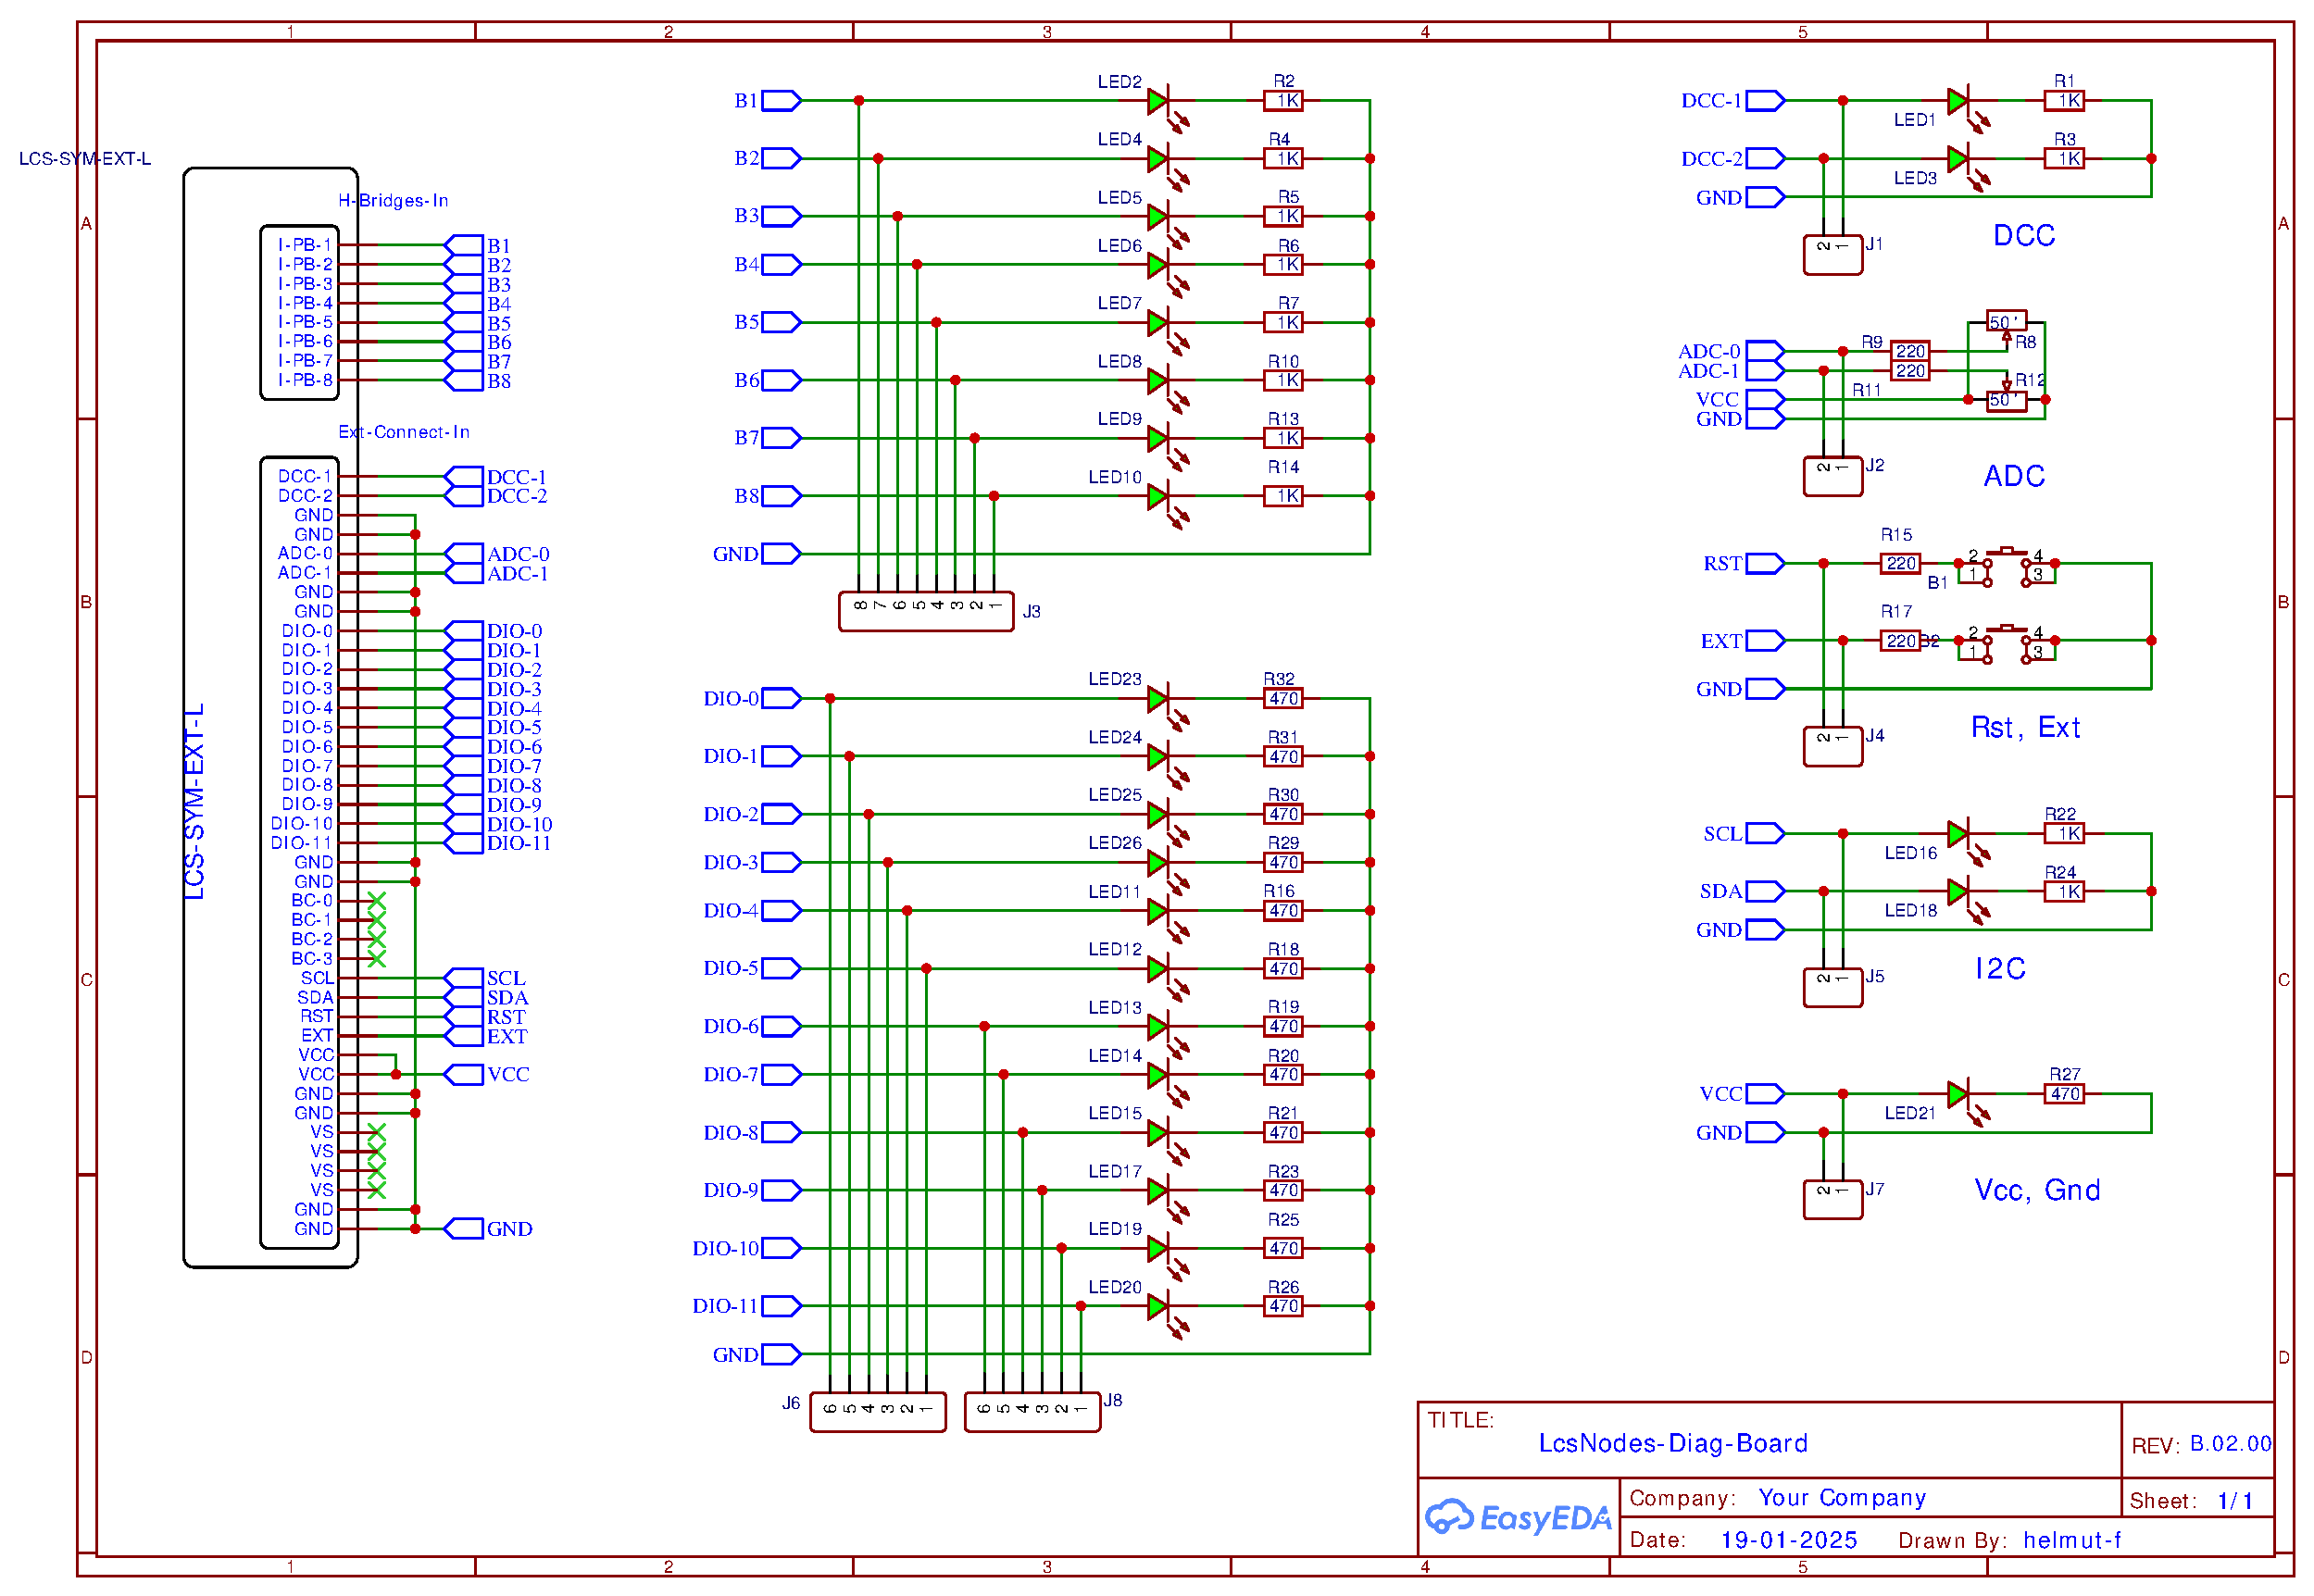
\includegraphics[page=1, width=0.7\textwidth]{./Schematics/Schematic_LcsNodes-Diagnostic-Board.pdf}
    \caption{Block Diagram}
    %\label{fig:schematic}
\end{figure}
\FloatBarrier

talk about the diagnostics. perhaps add the diagnostic program to the CDC or runtime library.

\section{BYE - Build your own extension}

It is often necessary to build rapid small prototypes, and this is where this board comes in handy.
BYE is an extension board featuring NVM logic and breadboard-style rows of holes for custom designs. 

\section{DCC bus to digital IO}

a small board for the DCC monitoring function to derive the DCC signal...

